\section{Results to date}
\label{sec:results}

The results below are organized by the validation ladder of Section~\ref{sec:datasets}. They are preliminary. Most were obtained on single spectra or small sets without replicate statistics, several rest on data that are not in the repository (the outputs of analysis runs are excluded from version control, and the raw Z300 shots reside on a laboratory file server), and none is an accuracy statement against a certified composition. Each number is traceable to a dated report, test, or document in the repository, cited in the source file next to the number. Where a later finding superseded an earlier one, the earlier value is not used.

\subsection{Synthetic round trips}

The first end-to-end test passed a Saha-consistent Ca/Mg scene (truth Ca~0.60, Mg~0.40, \SI{10}{\kilo\kelvin}, $\log_{10}\nel=17.0$) through the full pipeline. The baseline measured on 2026-07-16 was Ca~0.764, Mg~0.236 at \SI{7000}{\kelvin} with $r^2=0.509$ % src: tests/test_roundtrip_synthetic.py (module docstring)
, and a four-element quartz--carbonate scene lost its Si (truth 0.40) entirely while hallucinating Be at 0.23 with $\log_{10}\nel$ railed at 14.0, the lower search bound % src: bench/synth_cases.py (module docstring)
. These baselines were the floor from which the subsequent fixes were measured.

The stage-consistency thermometer (Section~\ref{sec:theory-thermometer}) was the first fix evaluated against them. Its diagnosis is the starting point: at fixed $T$ the data misfit is identical to four digits for $\log_{10}\nel$ between 14 and 18, and on both the Ca/Mg and silicate scenes the data prefer 5.5--\SI{7}{\kilo\kelvin} to the true \SI{10}{\kilo\kelvin} by less than 1\% in misfit % src: reports/2026-09-21-stage-consistency-thermometer.md (sec. 1)
. On the Ca/Mg scene the stage-tie cost has its global minimum at the truth node (360 in data units, against $2.6\times10^6$ at the state the amplitude objective alone had selected), but a Saha ridge runs through the surface along which a hotter plasma at higher $\nel$ gives the same ion fractions % src: reports/2026-09-21-stage-consistency-thermometer.md (sec. 3)
. Table~\ref{tab:synthetic} gives the effect on three scenes with the round-trip test's fast settings (single seed).

\begin{table}[t]
\centering
\footnotesize
\caption{Synthetic round trips before and after the stage-consistency thermometer, bounded $\nel$, and grid-seeded search. Truth temperatures are 10, 10, and \SI{9}{\kilo\kelvin}. $\tilde\epsilon$ is the median relative error on majors. Single seed, fast settings; reproduced from the dated report.}
\label{tab:synthetic}
\begin{tabular}{@{}lrrrr@{}}
\toprule
Scene & $T$ before (K) & $T$ after (K) & $\tilde\epsilon$ before & $\tilde\epsilon$ after \\
\midrule
Ca/Mg binary & 7000 & 8908 & 0.33 & 0.17 \\
Silicate, four elements & 7000 & 9043 & 0.66 & 0.53 \\
Feldspar-like & 7000 & 9242 & 0.80 & 0.18 \\
\bottomrule
\end{tabular}
% src: reports/2026-09-21-stage-consistency-thermometer.md (sec. 4 table and bullet list)
\end{table}

Two caveats accompany the table. The $\nel$ search box was set on these same synthetic scenes by grid search (a $2\sigma$ box left the Ca/Mg scene at its low edge with the wrong dominant element), so the scenes are not independent of the tuning % src: reports/2026-09-21-stage-consistency-thermometer.md (sec. 3)
. And the feldspar-like scene has no element with two observable ion stages, so its improvement comes entirely from the grid-seeded search and not from the thermometer. The iron-rich low-temperature case of Suite~S could not be rendered at the time of the report because its stage abundances summed to slightly less than one % src: reports/2026-09-21-stage-consistency-thermometer.md (What remains unverified)
; it has therefore not been used. The round-trip suite passed with 314 tests and 3 skipped at the time % src: reports/2026-09-21-stage-consistency-thermometer.md (sec. 4)
.

For the Stark channel, a synthetic test recovers $\log_{10}\nel$ to within 0.3 dex when the H$\alpha$ width coupling is active, and the same test asserts that $\nel$ is \emph{not} recovered when the coupling is switched off, ending near a search bound instead % src: tests/test_stark_ne.py (assertAlmostEqual delta=0.3; assertGreater/assertLess lines)
. This is the intended behavior and confirms that, without a width, $\nel$ is set by the prior.

\subsection{Engine benchmark}

A benchmark harness exists to score two inverse engines on identical NIST-backed synthetic spectra: the integrated peak-vector engine of this work, and a standalone full-spectrum variable-projection engine that had been developed as a prototype. The prototype was subsequently removed from the source tree after a module-by-module comparison found its core redundant with, and less complete than, the integrated engine; a small set of unadopted ideas was recorded for future A/B testing % src: docs/development_guide.md (Appendix, CF-LIBS prototype)
. No head-to-head scores are recorded in the repository, and the case generator of the harness still depends on the removed prototype, so the benchmark must be re-run with the in-repository generator before any engine comparison is reported. % searched reports/, docs/, notebooks/, DECISIONS.md, bench/ for recorded engine scores: none
The engine comparison is consequently an open item, not a result.

\subsection{Real-corpus behavior}

\paragraph{Effect of the thermometer on real spectra.}
On three real spectra without reference compositions (a vendor export, scan9x9, and REE\_44), the fitted temperature rose from 4.6--\SI{6.1}{\kilo\kelvin} to 7.3--\SI{8.6}{\kilo\kelvin} when the thermometer, grid-seeded search, and $\nel$ box were introduced, and the stage-tie cost fell by factors of 10 to 60. The residual $r^2$ was unchanged or slightly higher except for one spectrum (scan9x9), where it fell from 0.875 to 0.779 because, at the cold state, the fit had been good only because the stages were free % src: reports/2026-09-21-stage-consistency-thermometer.md (sec. 4)
. Two further spectra did not improve: REE\_01 had a negative $r^2$ before and after, and the argon spectrum stayed below $r^2=0.3$ while its temperature fell from \SI{12191}{\kelvin} to \SI{8563}{\kelvin}. The real samples (other than REE\_01) came out potassium-rich. The potassium support is the self-absorbed 766/\SI{770}{\nano\metre} resonance doublet, and the near-infrared amplitudes of two of the spectra rest on the fallback VIS-to-NIR response step, so the quality-control flags \texttt{dominant-weak-shape} and \texttt{detector-response-fallback} were set; the synthetic scenes, which have neither problem, are the evidence that state selection itself is sound. Without a reference composition, these real-sample results indicate that the physics terms moved the fits in the intended direction, not that they are accurate.

\paragraph{Confounder resolution.}
On the JChristensen set, Mn had been reported at 40--53\% atom fraction on the strength of two peaks inside the Mg~II doublet region. The contest of Eq.~\eqref{eq:contest} demoted both hot-Mn samples to \texttt{confounded} (contested share 1.0, confounder Mg), and resolution moved Mn from 53\% to 0\% and Mg from 8\% to 31\%, the latter being supported by an independent Mg~I line; Li, Al, and Ca detections with clear lines were unchanged apart from renormalization % src: docs/development_guide.md (Spectral confounders: Validated)
. In one pair, uncapped reattribution would have converted a 3.8\% Be confound into a 42\% Fe phantom (response ratio about 12); with the mass-creation guard Be retains its 3.8\% % src: docs/development_guide.md (Resolving the quantification, No mass creation)
. A first formulation based on the ratio of true-negative caps to demanded concentration failed by gutting genuine Li, which self-absorbs, and was discarded. A current-defaults re-run of all 38 JChristensen spectra finds Mn \texttt{confounded} on 6 and an upper limit on 10; Figure~\ref{fig:confounder} shows the \texttt{confounded} spectrum with the largest as-fit-to-resolved change.

\begin{figure*}[t]
\centering
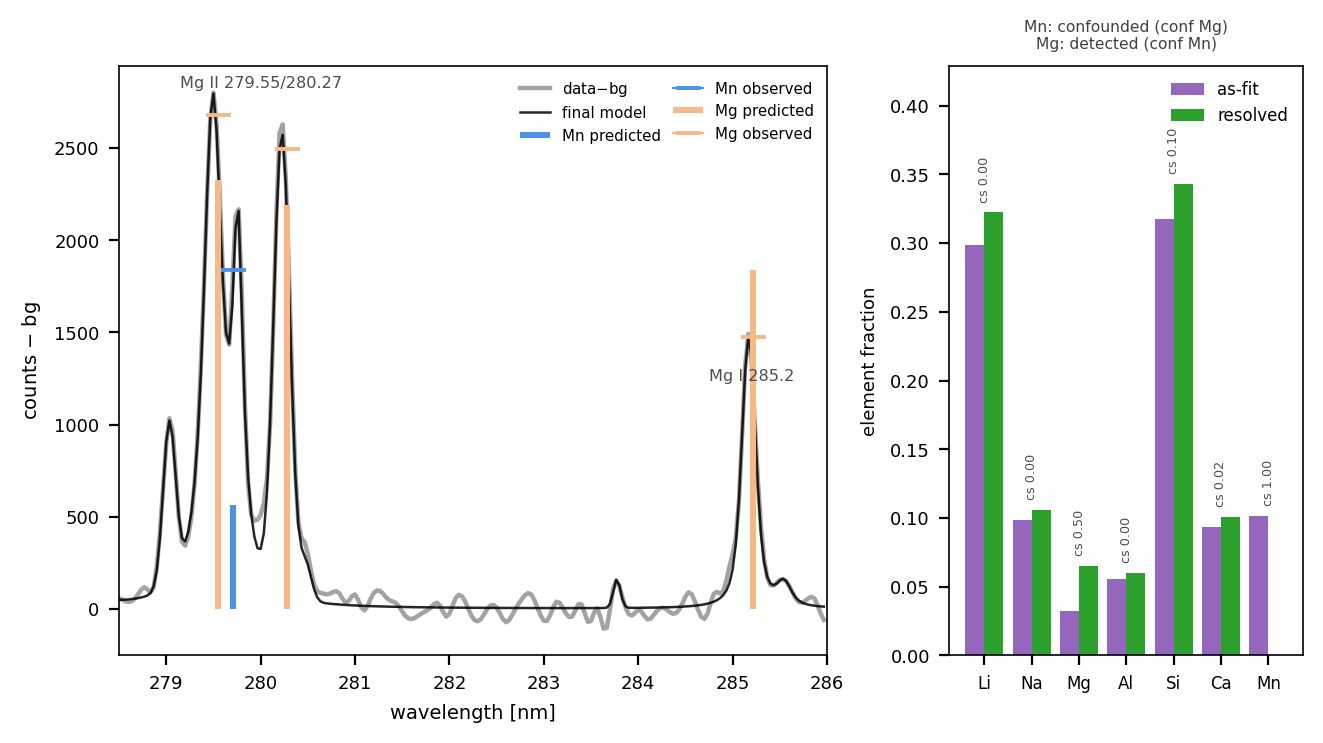
\includegraphics[width=\textwidth]{F4-confounder}
\caption{The Mn/Mg contest window (278.5--\SI{286}{\nano\metre}) of the JChristensen \texttt{MDD017-29-2c \#1} spectrum under the current adopted defaults. Left: background-subtracted data and final model; for each line that Mn or Mg claims, a stem gives that element's predicted amplitude and a bar marker the observed amplitude (areas converted to peak height). Mn's sole support line at \SI{279.76}{\nano\metre} predicts only about a third of the amplitude observed there, whereas Mg accounts for the Mg\,II 279.55/\SI{280.27}{\nano\metre} doublet and the independent Mg\,I \SI{285.2}{\nano\metre} line (which the model fits without the under-shoot seen on other spectra). Right: as-fit versus resolved fractions with the contested share (cs) above each element.
Of the 38 spectra, Mn is \texttt{confounded} on 6 and an upper limit on 10, 6 carry any \texttt{confounded} status, and the median $r^2$ is 0.78. On this spectrum ($T=\SI{9502}{\kelvin}$, $r^2=0.74$) Mn is fitted at 0.102 but its support is fully contested (cs~1.00, confounder Mg), so resolution moves Mn to 0.000 and Mg from 0.033 to 0.065. % src: manuscript/figures/cache/jc_mdd017_29_2c_1.json
\label{fig:confounder}}
\end{figure*}

\paragraph{Fit fidelity on MW2-112.}
On MW2-112 spectrum~1000, an earlier merge of asymmetric lines nearly doubled the global $\chi^2/\sigma^2$ (from 32\,821 to 51\,701) and left residuals of up to $+19\sigma$ and $40\sigma$. Replacing the merge by a nondestructive tag brought it to 28\,262, below the pre-merge value, and reduced unmodeled residuals above $3\sigma$ from 61 to 28 % src: docs/development_guide.md (Current status: ~85% complete, fit-fidelity review)
. On spectrum~0, the residual root-mean-square within merged-line windows is 2--8 times smaller for the self-absorption model than for the stored symmetric proxy for clean lines (Li~I 670.7: 227 vs 59; K~I 766.5: 101 vs 19; Fe 261.2: 141 vs 22), but is only modestly lower for a seven-component blend near \SI{383}{\nano\metre} (640 vs 549) % src: docs/fit_pipeline.md (table of merged-line residuals)
. Fit quality for blends is therefore not solved.

\paragraph{Absolute versus relative composition on MW2-112.}
In a 20-shot pilot of the closed-sum composition run, 19 nonzero spectra completed (the all-zero spectrum was correctly an error); only 3 passed quantitative physical quality control, 4 warned, and 12 failed because of low or negative $r^2$, parameters at bounds, or weak-shape and composition collapse. Doubling optimizer effort and varying the \SI{620}{\nano\metre} fallback response changed compositions substantially without stable improvement, and the 929-shot closed-sum run was rejected by the pre-registered gate % src: docs/mw2_112/analysis_plan.md (sec. 9)
. A relative-profile branch using 255 same-stage multiplets, matched-filter areas, and a requirement of at least two coherent lines per ion stage was completed for all 929 spectra. Its within-element rank correlation with the vendor summaries is 0.934 for Si, 0.883 for Ti, 0.705 for Fe, 0.657 for Li, and 0.598 for Mg, but 0.030 for Al, which is internally coherent yet externally discordant and is flagged as model limited % src: docs/mw2_112/provenance.md (Reported Spearman correlations); docs/mw2_112/analysis_plan.md (sec. 9)
. Because the vendor summaries are themselves uncalibrated, these correlations show agreement of trends, not correctness. An independent peak-window procedure supports ten elements (Al, Ba, Ca, Fe, Li, Mg, Na, Si, Sr, Ti) and rejected preliminary Ag, Cu, Ga, Ge, and V assignments as blends or single-line evidence % src: docs/mw2_112/analysis_plan.md (sec. 10)
. The output directories of these runs are not under version control.

\paragraph{A rejected physics change.}
Introducing the stimulated-emission factor into the optical depth left median $\Delta r^2$ and median change in stage disagreement at zero over 38 JChristensen spectra, yet changed alkali and Si compositions by more than 20\% in 14 of 38 samples (a control that perturbed only the optimizer trajectory did so in 3 of 38). It was refused as default because it reorients a near-degenerate alkali self-absorption and composition direction without adding information % src: docs/development_guide.md (Appendix, item 1, A/B result)
. This is an example of the acceptance logic of Section~\ref{sec:metrics}: neutral fit quality with large composition swings is instability, not accuracy.

\paragraph{Native-grid recovery.}
On the standard vendor export, which the $1/30$\,\si{\nano\metre} grid reproduces by cubic-spline resampling of the native detector pixels, the native knots were recovered to a relative residual below $10^{-6}$ in 99.1\%, 96.6\%, and 97.3\% of the NIR, VIS, and UV segments respectively across 7\,821 spectra, with a median residual of order $10^{-11}$; the \SI{0.1}{\nano\metre} export is a different product and is not covered % src: reports/2026-09-20-alibz-review.md (Moissanite archive runs table)
.

\subsection{Pure-element standards on the Z300}

Figure~\ref{fig:standard} applies the pipeline to a fresh-site iron standard on the 18-pixel-corrected native axis.

\begin{figure*}[t]
\centering
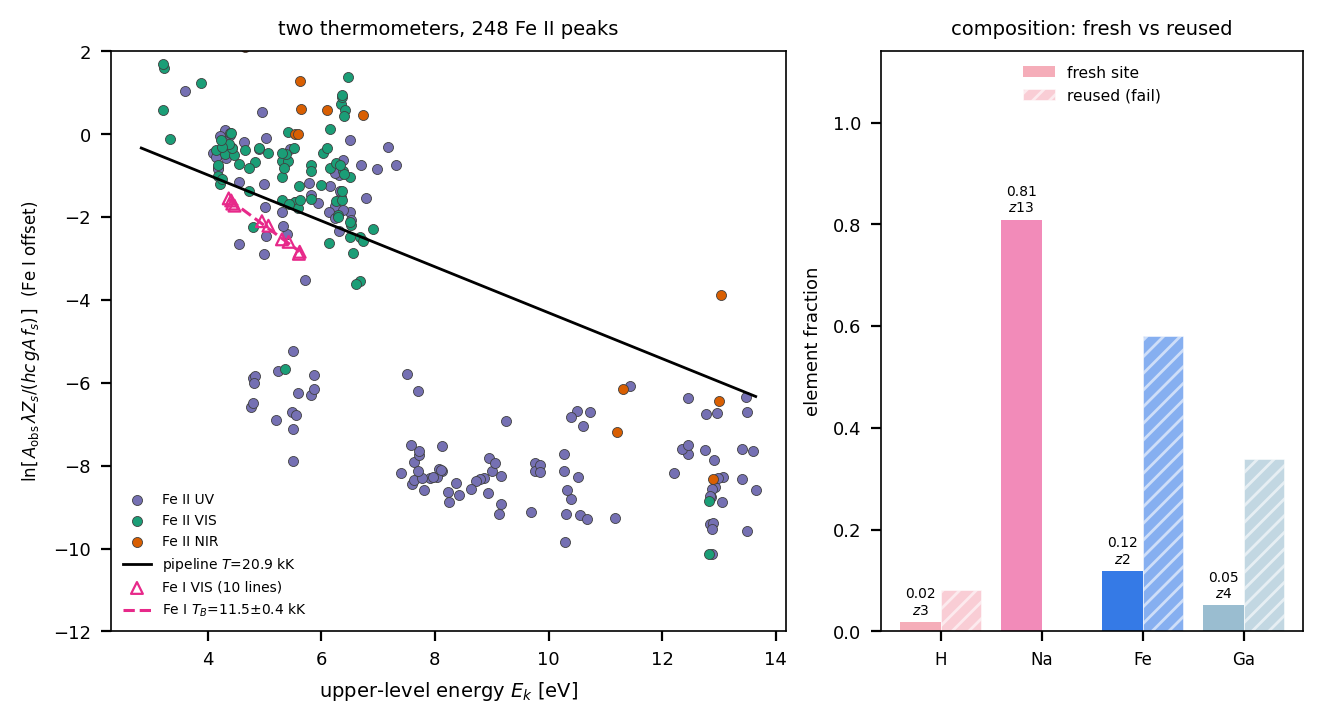
\includegraphics[width=\textwidth]{F5-standard}
\caption{Two thermometers on a pure-iron standard (\texttt{Fe\_aesar\_9998}, fresh raster site, delay 5, period 25) on the 18-pixel-corrected Z300 native axis. (a)~The whole-pattern solve's Boltzmann points, $\ln[A_{\mathrm{obs}}\,\lambda\,Z_s(T)/(hc\,gA\,f_s(T,n_e))]$ against upper-level energy $E_k$ (indexer \texttt{line\_emissivity} convention, Saha fraction $f_s$ divided out), coloured by detector segment, with the line of slope $-1/k_BT$ at the fitted $T$; the $y$-range is clipped to $[-12,2]$ (one point at $\ln\approx-20$ dropped). Overlaid are the line-selected Fe\,I visible lines (triangles, shifted vertically for display; only the slope is comparable) and their Boltzmann fit. (b)~composition, fresh (solid) versus reused spot (hatched), with detection $z$-scores.
The whole-pattern solve sits at $T=\SI{22601}{\kelvin}$ with $\log_{10}n_e=17.69$ at the upper bound of the H$\alpha$ box and assigns all 112 Fe peaks to Fe\,II (no Fe\,I), whereas the 10 isolated Fe\,I visible lines give $T_B=11.5\pm\SI{0.4}{\kilo\kelvin}$ ($r^2=0.99$, but over only a \SI{1.25}{\electronvolt} $E_k$ span, below the campaign's \SI{2.4}{\electronvolt} resolution threshold), consistent with the Fe\,I campaign median of \SI{10.8}{\kilo\kelvin}. The figure therefore documents the thermometer discrepancy on a target of known composition, not an inter-stage tie; the fresh site recovers Fe~0.93 ($z=315$, H~0.07), while the reused spot collapses to a spurious B~0.83 with Fe~0.17. % src: manuscript/figures/cache/fe_fresh_d5p25.json; manuscript/figures/cache/fe_reused_fail.json
\label{fig:standard}}
\end{figure*}

\paragraph{Axis correction.}
All Z300 native spectra were found to carry a fixed 18-pixel offset in the pixel-to-wavelength map, labeling lines about 1.6 (UV), 2.3 (VIS), and \SI{3.3}{\nano\metre} (NIR) too blue; it was identified by correlating spectra with predicted line sticks (best offsets $-18.5$, $-18.25$, and $-18.5$ pixels in the three segments) % src: reports/2026-09-23-native-axis-18px-offset.md (Finding; Evidence)
. After the correction the global shift of the Fe data is \SI{-22}{\pico\metre} (against \SI{-154}{\pico\metre} before), and a residual of about $-0.25$ pixel remains, with median manifest-recorded Ar~I offset of $-0.25$ pixel (range $-0.50$ to $+0.25$, 107 runs), varying with calibration epoch rather than constant % src: cal/reports/2026-09-24-fe-calibration-plasma-analysis.md (Wavelength shift model); reports/2026-09-24-wavelength-registration.md (Results)
. Every conclusion that depended on line identity in the earlier native analyses (registration engines, Ar anchor sets, within-segment slopes, Fe plasma temperatures, and self-absorption estimates) was repeated on the corrected axis, and only those repeated results are reported here. For example, the earlier conclusion that only three NIR Ar~I lines are argon, and the opposite-signed VIS slopes of Fe and V, were artifacts of the offset: on the corrected axis the VIS slope is about zero for both metals % src: reports/2026-09-24-wavelength-registration.md (Wavelength dependence table); docs/wavelength_registration.md (argon anchors); DECISIONS.md (2026-09-23 entries, superseded)
. Note that the 2026-09-23 entries in the decision log predate this correction.

\paragraph{Registration and drift.}
Across 107 analyzed runs (20 Fe, 87 V), element shifts are tens of picometers per segment. The best-sampled group (87 V runs over 22~h) shows a drift of about \SI{1}{\pico\metre\per\hour}, resolved statistically but physically small compared with the fixed offsets and the vendor recalibration step, so a warm-up drift hypothesis is not supported % src: reports/2026-09-24-wavelength-registration.md (Drift verdict)
. A vendor recalibration moved the Fe residual by 17--\SI{32}{\pico\metre} % src: reports/2026-09-24-wavelength-registration.md (Pre vs post the 13:39 recalibration)
.

\paragraph{Peak location.}
On 330 thin Fe lines (24 runs) in the VIS segment, the empirical point-spread-function (ePSF) estimator has a median absolute residual of \SI{5.3}{\pico\metre} against 11.2--\SI{12.3}{\pico\metre} for the vendor spline root and native parabola, with paired confidence intervals excluding zero. In the UV the spline and parabola win (4.7--\SI{4.8}{\pico\metre} against 7.6 for ePSF, on 118 thin Fe lines), and in the NIR, where there are no Fe lines, the ePSF wins on Ar~I (for 696.54~nm, 4.8 against 14--\SI{15}{\pico\metre}) but is gated to a point-Gaussian because of a sub-band seam bias % src: cal/reports/2026-09-24-empirical-lsf.md (sec. 3); alibz/data/epsf-z300-20260924.json (location blocks)
. The per-segment choice (spline in UV, ePSF in VIS, Gaussian in NIR) is therefore a measured one, and the UV and NIR entries rest on small or indirect samples.

\paragraph{Iron plasma.}
Iron-line matching on the corrected axis gives 86\% of peaks within \SI{0.15}{\nano\metre} of a database Fe line (95\% within \SI{0.40}{\nano\metre}), against 78\% and 88\% for V % src: cal/reports/2026-09-24-line-matching-sa-broadening.md (sec. 1.4)
. A Fe~I Boltzmann temperature in the visible resolves in 5 of 26 runs, giving 6873--\SI{13701}{\kelvin} (median \SI{10805}{\kelvin}) with per-run uncertainty about 15--25\%; the Fe~II UV fit resolves in none. The temperature is not detectably different across the delay/period grid (detection limit about \SI{421}{\kelvin}) and the Fe~II/Fe~I area ratio is 0.90--2.09 (median 1.49) % src: cal/reports/2026-09-24-fe-calibration-plasma-analysis.md (sec. 4 and conclusions)
. Before the axis correction the corresponding result was 8191--\SI{10451}{\kelvin} (median 9321~K) from 2 of 26 runs; the conclusion that the plasma belongs to the 8000--\SI{11000}{\kelvin} class survives, but the individual numbers do not % src: cal/reports/2026-09-24-fe-calibration-plasma-analysis.md (old versus corrected table)
. The McWhirter criterion gives only a lower bound, $\nel\ge10^{16}\,\mathrm{cm^{-3}}$ at \SI{10}{\kilo\kelvin} % src: cal/reports/2026-09-24-fe-calibration-plasma-analysis.md (4c)
, and no measured $\nel$ is reported because the cross-segment response is uncalibrated. Surface contamination (K~I) decays about 4.4-fold over the first few shots, so the first three shots on a fresh site are discarded for bulk work % src: cal/reports/2026-09-24-fe-calibration-plasma-analysis.md (discard recommendation)
.

\paragraph{Vanadium and optical depth.}
In the vanadium timing study the score falls monotonically with period at every delay (period means 1.234, 1.182, 1.119, 0.993 for periods 1, 10, 25, 50), but the V~I line signal is flat with period; the period-scaled background is a detector fixed pattern, not plasma continuum, so period acts as an exposure and the minimum period is preferred % src: cal/reports/2026-09-24-vanadium-timing-study.md (sec. 8, Q2)
. Delay is a genuine plasma lever: in an independent first run with a different site order, the V~II 311 line falls with delay at $-0.0252\pm0.0049$ per unit (5.1$\sigma$) while crater depth is not significant % src: cal/reports/2026-09-24-vanadium-timing-study.md (sec. 8, Q1)
. On the corrected axis, the temperature-independent V~I pair at 417.94/\SI{415.97}{\nano\metre} sits near its optically thin ratio (the thin value is about 2.05) and does not vary with period (its decrease with delay remains unexplained), whereas the earlier ratio of 0.75 interpreted as strong self-absorption was a misidentification caused by the offset % src: cal/reports/2026-09-24-vanadium-timing-study.md (sec. 8, Q3); reports/2026-09-23-native-axis-18px-offset.md
. This does not mean V is optically thin: the multiplet test selects seven usable V~I/II pairs, of which the strongest give optical depths of about 3.5, 1.4, and 1.4 for pairs 565.74/560.49, 653.14/645.23, and 609.02/\SI{603.97}{\nano\metre}, and 8 of 14 low-lying V~I lines lie well below the Boltzmann reference. Fe shows self-absorption on a few clean pairs (for instance 589.80/589.53 with $\tau\approx8.5$), which the earlier, misaligned analysis had found thin % src: cal/reports/2026-09-24-line-matching-sa-broadening.md (2a, 2e)
. The conclusion that pure-metal resonance lines are unsuitable as wavelength anchors, because the strongest lines are optically thick and displaced, stands from the earlier registration decision % src: DECISIONS.md (2026-09-23 independent wavelength registration)
.

\subsection{Literature-driven changes scored on a fixed panel}
\label{sec:results-ab}

Seven changes drawn from the literature of Section~\ref{sec:intro} were implemented behind
options that default off and scored, before and after, on one fixed panel: the five synthetic
suite-S scenes, the five real sample spectra, and the 26 run means of the iron standard
(Section~\ref{sec:datasets}), at the fast search settings, on one machine so that paired
comparisons are meaningful. % src: reports/2026-11-03-ab-wave1-verdicts.md; reports/fit-panel/*-moissanite.json
Table~\ref{tab:ab} gives the panel means. Huber reweighting of the concentration solve
\citep{huber1964robust} is worse on every panel. False-discovery-rate control of the element
detection score \citep{benjamini1995fdr} leaves the synthetic and real panels unchanged but
collapses the recovered iron fraction on the pure-iron standard (0.40 to 0.19) while removing the
spurious light elements, because the threshold over several hundred candidates rises above the
score of iron's own best line on runs where iron is already starved by the defect described next.
Adaptive non-negative LASSO \citep{tibshirani1996lasso,zou2005elasticnet} is neutral where it was
meant to act, since the synthetic spurious mass is already zero. The Debye correction to the
ionization energies (Section~\ref{sec:theory-saha}) is mixed. Tabulated partition functions
\citep{barklem2016partition} raise the recovered iron fraction on the standard from 0.40 to 0.56
(better on 15 of 26 runs, worse on 8) and are neutral on real spectra, but score slightly worse on
the synthetic scenes; with the Debye correction added they improve the real-spectrum $r^2$ on all
five spectra. % src: reports/2026-11-03-ab-wave1-verdicts.md

\begin{table}[t]
\centering
\footnotesize
\caption{Wave-1 panel means (fast settings; 5 synthetic, 5 real, 26 Fe-standard items; one machine).
Lower is better except $r^2$ and the Fe fraction. % src: reports/2026-11-03-ab-wave1-verdicts.md
}
\label{tab:ab}
\begin{tabular}{@{}lccccc@{}}
\toprule
Variant & Syn. median rel. err. & Syn. $|T|$ err. & Real $r^2$ & Real stage dis. & Fe fraction \\
\midrule
baseline & 0.207 & 0.082 & 0.471 & 0.515 & 0.404 \\
adaptive NN-LASSO & 0.204 & 0.081 & 0.469 & 0.467 & 0.441 \\
Huber IRLS & 0.375 & 0.197 & 0.371 & 0.496 & 0.334 \\
Debye IPD & 0.237 & 0.078 & 0.471 & 0.487 & 0.385 \\
partition tables & 0.218 & 0.085 & 0.466 & 0.491 & 0.559 \\
tables + IPD & 0.231 & 0.081 & 0.473 & 0.509 & 0.533 \\
FDR 0.05 (BH) & 0.207 & 0.082 & 0.471 & 0.515 & 0.186 \\
\bottomrule
\end{tabular}
\end{table}

The synthetic penalty of the partition tables was traced, not accepted. A scene rendered and
inverted with the same tables recovers Ca/Mg worse (median relative error 0.22) than the
line-sum pair (0.08), which a consistent forward and inverse pair should not do. The forward and
inverse models agree in emissivity space for both partition sources; the difference is in where
the plasma-state search lands. At the exact true state the inverse over-recovers Ca with either
source (0.63 line-sum, 0.71 tables, truth 0.60); the tables raise the Ca~\textsc{i} partition
function by about \SI{45}{\percent} near \SI{10}{\kilo\kelvin}, which moves the stage-consistency
minimum onto the true node where that bias is fully expressed, whereas the line-sum search lands
on a cold basin (\SI{8.9}{\kilo\kelvin}, $\log_{10}\nel=16.5$) where the bias is accidentally
compensated. % src: reports/2026-11-03-debug-partition-roundtrip.md
The bias itself was then isolated to the design matrix. Each database line's predicted emission
is spread over every fitted peak within the \SI{0.1}{\nano\meter} shift tolerance by a Voigt
height ratio, so one line can be counted against several peaks and a dense-forest element is
over-predicted per unit concentration in proportion to how often its lines fall near two fitted
components. With a fitter-realistic oracle (the forward model's own line areas, lines closer than a
quarter of the instrumental width merged into one peak as a fitter would merge them) solved at the
exact true state, the legacy map returns Si 0.31 and Ca 0.37 on the silicate scene (truth 0.40 and
0.30), whereas assigning each line to the single fitted component under it, so that a component is
the sum of the database lines it covers, returns 0.36 and 0.27; on the binary scene the two maps
give Ca 0.61 and 0.60. A clean control $\mathbf{y}=\mathbf{A}\mathbf{c}_\mathrm{true}$ is exact
under the hard assignment but not under the legacy map, which is therefore inconsistent even on
its own data. % src: reports/2026-11-04-candidate-coverage.md (merged oracle tables); reports/2026-11-03-wave2-conserving-design.md
The same oracle exposed a second, independent gap: iron is recovered at 0.27 (truth 0.20) under
either map because the design matrix under-predicts the generator's iron areas by about a factor
1.23 relative to the other elements at the same plasma state, so the solve inflates iron to
compensate; the per-element aggregation itself is exact on a clean control. The source of that
iron-specific forward-versus-inverse disagreement is being isolated. % src: reports/2026-11-04-aggregation-floor.md
Both the conserving and the hard-assignment maps were implemented as options and scored in a
second round together with the partition tables and the Debye correction, against a baseline built
from the same code (the panel is deterministic: identical code reproduces every metric). The
hard assignment is exact at the true state and clean of spurious species, but end to end, at the
fast search settings, it scores worse than the baseline on the synthetic median error (0.208 against
0.156) because the unweighted solve absorbs iron's line-shape misfit; the conserving map combined
with the tables and the Debye correction is the only variant that improves the mean of every
headline on all three panels. % src: reports/2026-11-04-ab-wave2-verdicts.md
Against the true baseline (a bisection found and gated two changes that had altered the default
path unflagged during the round, so every earlier comparison was re-run) the combination improves
every headline mean: synthetic median relative error 0.207 to 0.156 (better on three of five
scenes), temperature error 0.082 to 0.069, real-spectrum $r^2$ 0.471 to 0.478 and stage
disagreement 0.515 to 0.500 (each better on four of five spectra), and the iron fraction on the
pure-iron standard 0.40 to 0.55 (better on 13 of 26 runs). At the production search settings
the gains persist (synthetic median relative error 0.213 to 0.170, real $r^2$ 0.472 to 0.488,
iron fraction 0.43 to 0.56) with two costs we record: one synthetic scene's dominant element is
no longer identified correctly, and the spurious-element count on the iron standard rises
slightly (0.96 to 1.08), both within the paired noise of five- and 26-item panels. % src: reports/2026-11-04-ab-wave2-verdicts.md (series 3 + prod2); reports/fit-panel/{head,cpi}-prod2.json; DECISIONS.md 2026-11-04 addendum
These three options are now the pipeline defaults; the weighted solve with hard assignment, which
recovers every major of the silicate scene within 0.01 at the true state, remains an option
because its search misbehaves away from the true state.
A third round scored three further model changes behind flags, each against a baseline re-run on
the same tree. The overlap kernel was given each peak's own fitted width and each database line
its own Stark width at the trial electron density; at the fast search settings this variant lifted
the primary headline of every panel, but at the production settings it is mixed (real-spectrum
$r^2$ 0.489 to 0.509, better on four of five spectra, and the mis-identified dominant element of
the binary scene repaired, against synthetic median relative error 0.170 to 0.174 and iron fraction
0.563 to 0.545, worse on 14 of 26 runs), so it remains an option. The same round showed that the
merged oracle cannot arbitrate a width kernel at all, because its peaks sit on their own line
centres where every width gives unit overlap; only the end-to-end panel can. A bounded local polish
of the plasma state after the Bayesian search was rejected: a Powell polish within the budget is a
near no-op, and a Nelder--Mead polish lowers the outer objective by 10 to 60\% on the synthetic
scenes yet moves the temperature away from the truth, which says that the objective's minimum is
not at the true state and that a better search would not help until the model is. A two-temperature
stage thermometer (ion stages at $T+\delta$, $0 \le \delta \le 2000$~K) was rejected because
$\delta$ pins to its bound on three of five single-temperature synthetic scenes and doubles the
synthetic temperature error, and a per-species McWhirter gap flag changed no item on the panel
because the species it flags carry no multi-stage support. % src: reports/2026-11-04-w3-width-kernel.md; reports/2026-11-04-w3-outer-polish.md; reports/2026-11-04-w3-thermometer.md; reports/fit-panel/w3k-peakstark-conserve-prod.md

\subsection{Known failure modes}

The following failure modes were observed and are either guarded or flagged. None is claimed to be eliminated.

\begin{description}
\item[Basin collapse.] A re-index seeded with many weak low-excitation lines drifted into a low-temperature basin (about \SI{5200}{\kelvin}) where one element's small Saha--Boltzmann response explained everything, giving Hg~1.000 from a single \SI{194}{\nano\metre} line, Fe~0.991, and Ca~0.990 on JChristensen spectra, while $r^2$ rose to 0.87. A guard rejects a re-solve whose top fraction newly reaches 0.9 % src: docs/development_guide.md (honest measured caveat); alibz/pipeline.py (COLLAPSE_TOP_FRACTION comment)
.
\item[Phantom single-line elements.] Bi was reported at 0.94 when its strongest predicted line was 4 counts % src: docs/development_guide.md (A zero-emission species dominated the composition)
; in MW2-112, preliminary Ag, Cu, Ga, Ge, and V assignments were rejected as blends or single-line evidence % src: docs/mw2_112/analysis_plan.md (sec. 10)
. In a 99.98\% Fe target, almost every trace line lies near an Fe line, and several candidate trace detections (Ca~II, Ca~I) were downgraded to Fe-blends % src: cal/reports/2026-09-24-fe-calibration-plasma-analysis.md (sec. 1 table, limits)
.
\item[Confounders.] Mn$\leftrightarrow$Mg as above; a corpus-level catalog aggregates recurring pairs. An element whose all support is contested is an attribution choice, not a measurement.
\item[$\nel$ at bound.] The data lean cold along the Saha ridge, so the search sits at the low edge of whatever $\nel$ box it is given; for the reported vendor export the search ended at the H$\alpha$ edge and the exported flag \texttt{electron-density-at-bound} was set, together with \texttt{dominant-weak-shape} and \texttt{detector-response-fallback} % src: reports/2026-09-21-stage-consistency-thermometer.md (sec. 3 and sec. 4)
.
\item[Alkali resonance lines.] Rigid doublet-ratio vetoes are unsafe: 926 of 928 measured K pairs fall outside $\pm20\%$ of the thin ratio on the examined data, and K and Na compositions move by 30--60\% on real spectra with the self-absorption degeneracy % src: DECISIONS.md (2026-09-22 Early Ar/O diagnostics); docs/development_guide.md (Appendix item 1)
.
\item[Axis offset.] A fixed 18-pixel offset silently mis-assigned elements in all native Z300 data until 2026-09-24; an Ar~I cross-correlation check now records an axis warning in the acquisition record when the offset exceeds two pixels or the lock is ambiguous (it does not reject the data) % src: reports/2026-09-24-pixel-offset-fix.md (acquire.py axis check)
. Results from before the correction are superseded.
\end{description}

\subsection{Summary of evidence and gaps}

The evidence to date supports three statements. The inverse model, with the stage-consistency thermometer and an $\nel$ box, recovers the temperature and dominant composition of Saha-consistent synthetic scenes at the level of the pinned tolerances and moves real spectra to physically more plausible states. Confounded and collapsed solutions are detected and flagged, and some are resolved. And on pure-element standards the corrected axis, the line identifications, and a visible-range Boltzmann temperature are consistent with a plasma of roughly 7--\SI{14}{\kilo\kelvin}. The evidence does not yet support any statement about composition accuracy on real samples, the relative merit of the two inverse engines, or invariance to argon versus air. Those require certified reference materials, a re-run of the benchmark, and a dedicated paired acquisition, respectively (Section~\ref{sec:datasets}).
